\documentclass{standalone}

\begin{document}

\section{Experimental Evaluation}\label{evam}

\subsection{Hyperparameter Tuning}

Hyper-parameters are parameters that are not directly learnt within estimators. Hyperparameter settings could have a big impact on the prediction accuracy of the trained model. Optimal hyperparameter settings often differ for different datasets\cite{Alice:2015:Evaluating}.

\begin{itemize}
    \item Grid Search, which is commonly accepted as naive
because the number of required samples grows exponentially
in dimension, assuming the number of points per axis is held fixed. Though most expensive in terms of total computation time, if run in parallel, it is fast in terms of wall clock time.
\cite{lavalle2004relationship} has provided some insights into the relationship between
classical grid search and probabilistic roadmaps.

\item Random Search, which is a slightly variation on grid search. In stead of searching over the entire grid, random search only evaluates a random sample of points on the grid.
\cite{bergstra2012random} has shown that random search is  more efficient than grid search for hyper-parameter optimization
in the case of several learning algorithms on several data sets.
\end{itemize}

Scikit-learn provides both Exhaustive Grid Search\cite{scikit:grid} and Randomized Parameter Optimization\cite{scikit:random} class. To gain more insight about the hyperparameter tuning process (though might be useless), we used \href{http://scikit-learn.org/stable/modules/generated/sklearn.model_selection.ParameterGrid.html#sklearn.model_selection.ParameterGrid}{\verb|ParameterGrid} in our implementations. Test results of all parameter sets are included in log files. \verb||

\subsection{Evaluation Metrics}

% \scriptsize{
% What are criteria you are using to evaluate your method? What specific
% hypotheses does your experiment test? Describe the experimental methodology
% that you used. What are the dependent and independent variables? What is the
% training/test data that was used, and why is it realistic or interesting?
% Exactly what performance data did you collect and how are you presenting and
% analyzing it? Comparisons to competing methods that address the same problem
% are particularly useful. 
% }\normalsize

We used per-class accuracy, AUC and Normalized Gini Coefficient to evaluate out model.

\subsubsection{Per-Class Accuracy}

Accuracy simply measures how often the classifier makes the correct prediction. It’s the ratio between the number of correct predictions and the total number of predictions (the number of data points in the test set)\cite{Alice:2015:Evaluating}:
\begin{IEEEeqnarray}{C} 
accuracy = \frac{\mathrm{\#\ correct\ predictions}}{\mathrm{\#\ total\ data\ points}}\IEEEnonumber
\end{IEEEeqnarray}

Per-class accuracy is the average of the accuracy for each class. By using per-class accuracy, we can have a better understanding of the model if the target class was dominated by one label.

\subsubsection{Normalized Gini Coefficient and AUC}

The Normalized Gini coefficient, (named for the similar Gini coefficient/index used in Economics, which originally developed by Italian statistician and sociologist Corrado Gini\cite{Gini:1912}), measures the inequality among values of a frequency distribution (for example, levels of income)\cite{Gini:Wikipedia}. It is most commonly defined as twice the area between the ROC curve and the diagonal (with this area being taken as negative in the rare event that the curve lies below the diagonal)\cite{10.2307/1924845}.

\Cref{gini_graph} shows that the Gini coefficient is equal to the area marked $A$ divided by the sum of the areas marked $A$ and $B$, that is, $Gini = A / (A + B)$. It is also equal to $2A$ and to $1 - 2B$ due to the fact that $A + B = 0.5$ (since the axes scale from 0 to 1).

\begin{figure}[!t]
\centering
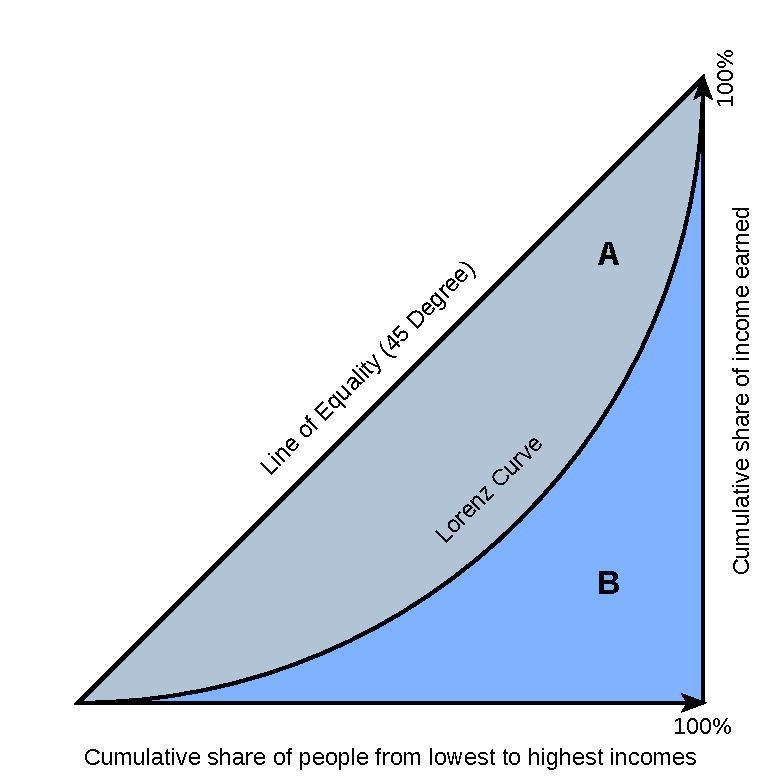
\includegraphics[width=.45\textwidth]{fig/gini.pdf}
\caption{Graphical Representation of the Gini Coefficient}
\label{gini_graph}
\end{figure}

The normalized Gini coefficient and AUC are closely related. AUC stands for area under the curve.
When using normalized units, the AUC is equal to the probability that a classifier will rank a randomly chosen positive instance higher than a randomly chosen negative one (assuming `positive' ranks higher than `negative')\cite{Fawcett:2006:IRA:1159473.1159475}. Elementary geometry shows that 
\begin{IEEEeqnarray}{C} 
Gini = 2 \times \mathrm{AUC} - 1.
\end{IEEEeqnarray}

The competition used normalized Gini coefficient to measure participants' submission performance. In our experiment, we worked in terms of both Gini coefficient and AUC.

\subsection{Evaluation Mechanisms}

% \subsubsection{K-Fold Cross-Validation}

We use $k$-fold cross-validation as our validation technique.

In $k$-fold cross-validation, we first divide the training dataset into $k$ folds. For a given hyperparameter setting, each of the $k$ folds takes turns being the hold-out validation set; a model is trained on the rest of the $k - 1$ folds and measured on the held-out fold. The overall performance is taken to be the average of the performance on all $k$ folds. Repeat this procedure for all of the hyperparameter settings that need to be evaluated, then pick the hyperparameters that resulted in the highest $k$-fold average.

Scikit learn provides multiple variations of $k$-fold\cite{scikit-learn}, for example, 
\begin{itemize}
    \item \href{http://scikit-learn.org/stable/modules/generated/sklearn.model_selection.KFold.html#sklearn.model_selection.KFold}{\verb|KFold}, which divides all the samples in k groups of samples, called folds of equal sizes (if possible). The prediction function is learned using $k - 1$ folds, and the fold left out is used for test.
    \item \href{http://scikit-learn.org/stable/modules/generated/sklearn.model_selection.LeaveOneOut.html#sklearn.model_selection.LeaveOneOut}{\verb|LeaveOneOut}, which is basically special simple case when $k = n$ in \verb|KFold|.
    \item \href{http://scikit-learn.org/stable/modules/generated/sklearn.model_selection.StratifiedKFold.html#sklearn.model_selection.StratifiedKFold}{\verb|StratifiedKFold}, which returns \emph{stratified} folds, i.e., each set contains approximately the \emph{same} percentage of samples of each target class as the complete set.
\end{itemize}

We chose \verb|StratifiedKFold| in out implementations during training phase.

\subsection{Results}
The best parameters of each model in our experiment is shown in \cref{performance}.

\begin{table*}[!t]
\centering
\caption{Performance of Each Models}\label{performance}
\begin{tabular}{llcc}
\toprule
\bfseries Model & \bfseries Optimal Parameters &Public Dataset & Private Dataset\\\midrule
Gradient Boost & \verb|'loss': 'deviance', 'max_depth': 4, 'n_estimators': 200| & 0.283 & 0.277  \\\hline
\multirow{2}{*}{Logistic Regression} & \verb|'C': 0.1, 'fit_intercept': False, 'penalty': 'l1'| & \multirow{2}{*}{0.266} & \multirow{2}{*}{0.257}  \\
& \verb|'random_state': 0, 'solver': 'liblinear'| &  & \\\hline
\multirow{2}{*}{Random Forest} & \verb|'bootstrap': False, 'criterion': 'entropy', 'max_depth': 10| & \multirow{2}{*}{0.263} & \multirow{2}{*}{0.258} \\
& \verb|'n_estimators': 40, 'warm_start': False| &&\\\bottomrule
\end{tabular}
\end{table*}

The result in public dataset performs best in \emph{Gradient Boosting}, then it is almost same for \emph{Logistic Regression} and \emph{Random Forest}. It is the same on private dataset.

Weak learners have high bias and low variance. For a decision tree, the weak learners are shallow trees and sometimes just stumps. Boosting mainly reduces bias to reduce error. On the other hand, \emph{Random Forest} tackles error by reducing variance in the opposite way as \emph{Gradient Boosting} does. As a result, it cannot deal with bias.
\emph{Logistic Regression} is some way like Gradient Boosting. It depends on the data set and type of features to know which model performs better.

For getting the best result, we adjusted the max depth of \emph{Gradient Boosting} to 4 after times of attempts, and since this model works well for overfitting we set the estimator to higher value as 200. We also used the `deviance' value for the loss parameter to optimize the lost function just like the way \emph{Logistic Regression}. This may get the conclusion that the comparison of \emph{Gradient Boosting} and \emph{Logistic Regression} depends on the dataset and features.

In \emph{Logistic Regression}, we set the C parameter to only $0.1$ to inverse the regularization strength to prevent overfitting. The random state is set to $0$ to control the random for every attempt to get the same and best result, compared to not setting random state or other state values, when dividing training set and testing set, avoid mess when in the next attempt. The parameter of \verb|solver| is set to \verb|liblinear| to work with the \verb|l1| penalty, at the same time, this problem is not a multiclass problem so there is no need to use other values of this parameter.

For the model of \emph{Random Forest}, the maximum depth is set to a number, not infinite by default to save running time however may be the reason why \emph{Random Forest} is a little worse than \emph{Gradient Boosting}. Other parameter is the best after many attempts to the best classification result.

\end{document}
